% %% %%%%%%%%%%%%%%%%%%%%%%%%%%%%%%%%%%%%%%%%%%%%%%%%%%%%%%%%%%
% practica.tex
%
% Author:  Mauricio Matamoros
% License: MIT
%
% %% %%%%%%%%%%%%%%%%%%%%%%%%%%%%%%%%%%%%%%%%%%%%%%%%%%%%%%%%%%

% TEX-ROOT=references.bib
% CHKTEX-FILE 1
% CHKTEX-FILE 13
\documentclass[letterpaper,10.5pt]{article}
% %% %%%%%%%%%%%%%%%%%%%%%%%%%%%%%%%%%%%%%%%%%%%%%%%%%%%%%%%%%
%
% packages.tex
%
%  Author: Mauricio Matamoros
%  Date:   2020.02.28
%
%  Contiene la lista de paquetes requeridos para generar
%  el archivo-reporte de las prácticas de laboratorio
%
% %% %%%%%%%%%%%%%%%%%%%%%%%%%%%%%%%%%%%%%%%%%%%%%%%%%%%%%%%%%
% Archivo principal de LaTeX
%!TEX root = ../reporte.tex

\usepackage[utf8]{inputenc}                  % Soporte para utf8
\usepackage[T1]{fontenc}                     % Soporte extendido de caracteres unicode
\usepackage[english,spanish,mexico]{babel}   % Define el idioma del documento a español (México) con soporte para inglés
% Standard packages
\usepackage{float}                           % Imágenes flotantes en el documento
\usepackage{ifthen}                          % Soporte if-then en macros
\usepackage{xspace}                          % Soporte de autoespaciado en macros
\usepackage{xstring}                         % Operaciones con cadenas en macros
\usepackage{wrapfig}                         % Permite colocar texto al rededor de figuras y otros flotantes
\usepackage{booktabs}                        % Embellece tablas
\usepackage{csquotes}                        % Entrecomillado automático y manejo de citas textuales
\usepackage{fancyhdr}                        % Permite reconfigurar encabezado y pie de página
\usepackage{fancyvrb}                        % Define estilos para entornos Verbatim
\usepackage{geometry}                        % Permite reconfigurar la geometría del documento
\usepackage{graphicx}                        % Permite insertar imágenes en varios formatos
\usepackage{lastpage}                        % Referencia a la última página del documento
\usepackage{listings}                        % Define estilos para entornos de código de programación (sintaxis)
\usepackage{multicol}                        % Manejo de texto en varias columnas
\usepackage{tabularx}                        % Tablas con ancho de columna variable
\usepackage{algorithm}                       % Entorno para escribir algoritmos
\usepackage{algpseudocode}                   % Entorno para escribir algoritmos en pseudocódigo
\usepackage[justification=centering]{subcaption} % Permite imágenes en viñetas
\usepackage[all]{nowidow}                    % Control de viudas y huérfanas
\usepackage[inline]{enumitem}                % Añade opciones de configuración a listas
\usepackage[usenames,dvipsnames]{xcolor}     % Permite el uso de colores en el documento
% Referencing
\usepackage{varioref}                        % Gestión de referencias variables
\usepackage{hyperref}                        % Gestión de referencias e hipervínculos
\usepackage[noabbrev,nameinlink,spanish]{cleveref} % Gestión de referencias cruzadas inteligentes con hipervínculos
\usepackage[square, comma, numbers, sort&compress]{natbib} % Gestión de referencias bibliográficas

% %% %%%%%%%%%%%%%%%%%%%%%%%%%%%%%%%%%%%%%%%%%%%%%%%%%%%%%%%%%
%
% macros.tex
%
%  Author: Mauricio Matamoros
%  Date:   2020.02.28
%
%  Contiene los macros personalizados definidos para
%  el archivo-reporte de las prácticas de laboratorio
%
% %% %%%%%%%%%%%%%%%%%%%%%%%%%%%%%%%%%%%%%%%%%%%%%%%%%%%%%%%%%
% Archivo principal de LaTeX
%!TEX root = ../reporte.tex

%CHKTEX-FILE 9
%CHKTEX-FILE 21

\newcommand{\lpar}{(}
\newcommand{\rpar}{)}
\newcommand{\textcommand}[1]{\texttt{\textbackslash#1\{\}}}
\newcommand{\textenviron}[2][y]{\texttt{\textbackslash{}begin\{#2\} #1 \textbackslash{}end\{#2\}}}


\input{setup/colorboxes}
%CHKTEX-FILE 1
%CHKTEX-FILE 7
%CHKTEX-FILE 9
% Default fixed font does not support bold face
\DeclareFixedFont{\ttb}{T1}{txtt}{bx}{n}{8} % for bold
\DeclareFixedFont{\ttm}{T1}{txtt}{m}{n}{8}  % for normal

% Custom colors
\usepackage{color}
\definecolor{keywordsColor}{rgb}{0,0,0.5}
\definecolor{customColor}{rgb}{0.6,0,0}
\definecolor{stringColor}{rgb}{0,0.5,0}

% Code highlighting python
\renewcommand{\ttdefault}{pcr}
\lstset{
	language=Python,                              % the language of the code (can be overrided per snippet)
	backgroundcolor=\color{white},                % choose the background color
	basicstyle=\footnotesize\ttfamily,            % the size of the fonts that are used for the code
	breakatwhitespace=false,                      % sets if automatic breaks should only happen at whitespace
	breaklines=true,                              % sets automatic line breaking
	captionpos=t,                                 % sets the caption-position to bottom
	commentstyle=\color{gray},                    % comment style
	deletekeywords={},                            % if you want to delete keywords from the given language
%	escapeinside={\%*}{*)},                       % if you want to add LaTeX within your code
	extendedchars=true,                           % lets you use non-ASCII characters; for 8-bits encodings only, does not work with UTF-8
	frame=tb,                                     % adds a frame around the code
	keepspaces=true,                              % keeps spaces in text, useful for keeping indentation of code (possibly needs columns=flexible)
	keywordstyle=\color{keywordsColor}\bfseries,  % keyword style
	numbers=left,                                 % where to put the line-numbers; possible values are (none, left, right)
	numbersep=5pt,                                % how far the line-numbers are from the code
	numberstyle=\tiny\color{gray},                % the style that is used for the line-numbers
	rulecolor=\color{black},                      % if not set, the frame-color may be changed on line-breaks within not-black text (e.g. comments (green here))
	showspaces=false,                             % show spaces everywhere adding particular underscores; it overrides 'showstringspaces'
	showstringspaces=false,                       % underline spaces within strings only
	showtabs=false,                               % show tabs within strings adding particular underscores
	stepnumber=1,                                 % the step between two line-numbers. If it's 1, each line will be numbered
	stringstyle=\color{stringColor},              % string literal style
	tabsize=2,                                    % sets default tabsize to 2 spaces
	title=\lstname,                               % show the filename of files included with \lstinputlisting; also try caption instead of title
	columns=fixed,                                % Using fixed column width (for e.g. nice alignment)
	otherkeywords={self},                         % if you want to add more keywords to the set
	emphstyle=\color{customColor}\bfseries,       % Custom highlighting style
	emph={__init__,__main__,True,False,None},     % Custom highlighting keywords
	xleftmargin=1cm,                              % Left margin
	xrightmargin=1cm,                             % Right margin
	% Unicode compatibility
	inputencoding=utf8,
	literate={%
	            {Á}{{\'a}}1 {É}{{\'E}}1 {Í}{{\'I}}1 {Ó}{{\'O}}1 {Ú}{{\'U}}1%
	            {á}{{\'a}}1 {é}{{\'e}}1 {í}{{\'i}}1 {ó}{{\'o}}1 {ú}{{\'u}}1%
	            {À}{{\`A}}1 {È}{{\'E}}1 {Ì}{{\`I}}1 {Ò}{{\`O}}1 {Ù}{{\`U}}1%
	            {à}{{\`a}}1 {è}{{\`e}}1 {ì}{{\`i}}1 {ò}{{\`o}}1 {ù}{{\`u}}1%
	            {Ä}{{\"A}}1 {Ë}{{\"E}}1 {Ï}{{\"I}}1 {Ö}{{\"O}}1 {Ü}{{\"U}}1%
	            {ä}{{\"a}}1 {ë}{{\"e}}1 {ï}{{\"i}}1 {ö}{{\"o}}1 {ü}{{\"u}}1%
	            {Â}{{\^A}}1 {Ê}{{\^E}}1 {Î}{{\^I}}1 {Ô}{{\^O}}1 {Û}{{\^U}}1%
	            {â}{{\^a}}1 {ê}{{\^e}}1 {î}{{\^i}}1 {ô}{{\^o}}1 {û}{{\^u}}1% CHKTEX 19
	            {Ã}{{\~a}}1 {Ẽ}{{\~E}}1 {Ĩ}{{\~I}}1 {Õ}{{\~O}}1 {Ũ}{{\~U}}1 {Ñ}{{\~N}}1%
	            {ã}{{\~a}}1 {ẽ}{{\~e}}1 {ĩ}{{\~i}}1 {õ}{{\~o}}1 {ũ}{{\~u}}1 {ñ}{{\~n}}1%
	            {œ}{{\oe}}1 {Œ}{{\OE}}1 {æ}{{\ae}}1 {Æ}{{\AE}}1 {ß}{{\ss}}1%
	            {ç}{{\c c}}1 {Ç}{{\c C}}1 {ø}{{\o}}1 {å}{{\r a}}1 {Å}{{\r A}}1%
	            {€}{{\EUR}}1 {£}{{\pounds}}1 {×}{{\(\times\)}}1% CHKTEX 21
	            {°}{{\textsuperscript{o}}}1%
	            {¹}{{\textsuperscript{1}}}1%
	            {²}{{\textsuperscript{2}}}1%
	            {³}{{\textsuperscript{3}}}1%
	            {⁴}{{\textsuperscript{4}}}1% CHKTEX 19
	            {⁵}{{\textsuperscript{5}}}1% CHKTEX 19
	            {⁶}{{\textsuperscript{6}}}1% CHKTEX 19
	            {⁷}{{\textsuperscript{7}}}1% CHKTEX 19
	            {⁸}{{\textsuperscript{8}}}1% CHKTEX 19
	            {⁹}{{\textsuperscript{9}}}1% CHKTEX 19
	            {⁰}{{\textsuperscript{0}}}1% CHKTEX 19
%	            {A}{{\textAlpha}}1
	            {α}{{\textalpha}}1%
%	            {B}{{\textBeta}}1
	            {β}{{\textbeta}}1%
	            {Γ}{{\textGamma}}1
	            {γ}{{\textgamma}}1%
	            {Δ}{{\textDelta}}1
	            {δ}{{\textdelta}}1% CHKTEX 19
%	            {E}{{\textEpsilon}}1
	            {ϵ}{{\textepsilon}}1%
%	            {Z}{{\textZeta}}1
	            {ζ}{{\textzeta}}1%
%	            {H}{{\textEta}}1
	            {η}{{\texteta}}1%
	            {Θ}{{\textTheta}}1
	            {θ}{{\texttheta}}1%
%	            {I}{{\textIota}}1
	            {ι}{{\textiota}}1%
%	            {K}{{\textKappa}}1
	            {κ}{{\textkappa}}1%
	            {Λ}{{\textLambda}}1
	            {λ}{{\textlambda}}1%
%	            {M}{{\textMu}}1
	            {μ}{{\textmu}}1%
%	            {N}{{\textNu}}1
	            {ν}{{\textnu}}1%
	            {Ξ}{{\textXi}}1
	            {ξ}{{\textxi}}1%
%	            {O}{{\textOmikron}}1
%	            {o}{{\textomikron}}1%
	            {Π}{{\textPi}}1
	            {π}{{\textpi}}1%
%	            {P}{{\textRho}}1
	            {ρ}{{\textrho}}1%
	            {Σ}{{\textSigma}}1
	            {σ}{{\textsigma}}1%
%	            {T}{{\textTau}}1
	            {τ}{{\texttau}}1%
	            {ϒ}{{\textUpsilon}}1
	            {υ}{{\textupsilon}}1%
	            {Φ}{{\textPhi}}1
	            {ϕ}{{\textphi}}1%
%	            {X}{{\textChi}}1
	            {χ}{{\textchi}}1%
	            {Ψ}{{\textPsi}}1
	            {ψ}{{\textpsi}}1%
	            {Ω}{{\textOmega}}1
	            {ω}{{\textomega}}1%
	            {ζ}{{\varsigma}}1%
%	            {}{{\straightphi}}1%
%	            {}{{\scripttheta}}1%
%	            {}{{\straighttheta}}1%
%	            {}{{\straightepsilon}}1%
	         },
}

\lstdefinestyle{c_with_comments}%
{
	language     = c,
	morecomment  = [l]{//},
	morecomment  = [s]{/*}{*/},
	breaklines,
}

\lstdefinestyle{c_without_comments}%
{
	style        = c_with_comments,
	% numbers      = none,
	% keepspaces   = false,
	morecomment  = [l][\nullfont]{//},
	morecomment  = [is]{//}{\^^M},
	morecomment  = [is]{/*}{*/},
}

\lstdefinelanguage{conf}
{
	basicstyle=\ttfamily\small,
	columns=fullflexible,
	morecomment=[s][\color{Orchid}\bfseries]{[}{]},
	morecomment=[l]{\#},
	morecomment=[l]{;},
	commentstyle=\color{gray}\ttfamily,
	% morekeywords={},
	% otherkeywords={=,:},
	% keywordstyle={\color{Green}\bfseries}
}

% \captionsetup[lstlisting]{font={small,tt}}
\captionsetup[lstlisting]{%
	font={small},
}



\DefineVerbatimEnvironment{Verbatim}{Verbatim}{%
	fontsize=\footnotesize,%
	frame=leftline,%
	framesep=2em,    % separation between frame and text
}

\RecustomVerbatimCommand{\VerbatimInput}{VerbatimInput}{%
	fontsize=\footnotesize,
%	frame=lines,            % top and bottom rule only
	frame=leftline,         % left rule only
	numbers=left,           % Line numbers on the left
	numbersep=0.25em,       % Gap between numbers and verbatim lines
	xleftmargin=4em,        % Indentation to add at the start of each line
	xrightmargin=4em,       % Right margin to add after each line
	framesep=0.5em,         % separation between frame and text
	rulecolor=\color{Gray}, % Color of the lines
	labelposition=topline,  %
	samepage=false,         % When true, prevents verbatim environment from
	                        % being broken between pages
%	commandchars=\|\(\),    % escape character and argument delimiters for
	                        % commands within the verbatim
%	commentchar=*           % comment character
}


\hypersetup{
	hidelinks,
	colorlinks=true,
	linkcolor=Blue,
	filecolor=OliveGreen,
	urlcolor=RoyalPurple,
	pdfauthor={Mauricio Matamoros},
%	pdftitle={Práctica 0X – Fundamentos de Sistemas Embebidos},
% 	pdfsubject={The Subject},
% 	pdfkeywords={Some Keywords},
% 	pdfproducer={Latex with hyperref, or other system},
% 	pdfcreator={pdflatex, or other tool}
}

\captionsetup{%
	font=small
}

\geometry{%
	margin=2cm,
	% top=3cm,
	bottom=3cm,
	% left=2cm,
	% right=2cm,
	% inner=2cm,
	% outer=2cm,
	% headheight=,
	% footsep=,
	% footskip=,
}

\pagestyle{fancy}
\renewcommand{\headrulewidth}{0.0pt}
\lhead{}
\chead{}
\rhead{}
\lfoot{}
\cfoot{}
\rfoot{Página~\thepage~de~\pageref{LastPage}}

\crefname{table}{tabla}{tablas}
\Crefname{table}{Tabla}{Tablas}
\crefname{section}{sección}{secciones}
\Crefname{section}{Sección}{Secciones}
\crefname{subsection}{subsección}{subsecciones}
\Crefname{subsection}{Subsección}{Subsecciones}
\crefname{listing}{código de ejemplo}{códigos de ejemplo}
\Crefname{listing}{Código de Ejemplo}{Códigos de Ejemplo}
\renewcommand*{\lstlistingname}{Código ejemplo}


\author{\footnotesize Autor: José Mauricio Matamoros de Maria y Campos}
\title{Práctica 8:\\Control de temperatura en lazo cerrado\\de una lámpara incandecente\\usando Arduino y la Raspberry Pi\\
{\large Fundamentos de Sistemas Embebidos}}
\date{}

% Document body
\begin{document}
\maketitle

\section{Objetivo}%
\label{sec:objective}
El alumno aprenderá a controlar la temperatura de un entorno cerrado calentado una carga resistiva de alta potencia opto-acoplada a un microcontrolador por medio de un detector de cruce por cero, un TRIAC, y un sensor de temperatura LM35.

% %% %%%%%%%%%%%%%%%%%%%%%%%%%%%%%%%%%%%%%%%%%%%%%%%%%%%%%%%%%%
% intro.tex
%
% Author:  Mauricio Matamoros
% License: MIT
%
% %% %%%%%%%%%%%%%%%%%%%%%%%%%%%%%%%%%%%%%%%%%%%%%%%%%%%%%%%%%%

%!TEX root = ../practica.tex
%!TEX root = ../references.bib

\section{Introducción}%
\label{sec:introduction}
Existen múltiples herramientas para desarrollar sistemas embebidos, tales como
	Buildroot~\Citep{buildrootManual,barry2012modern},
	Yocto Project~\Citep{yoctoManual,barry2012modern}
	y
	Linaro Project~\Citep{barry2012modern},
entre otros.
De estos se ha elegido Buildroot por ser minimalista y sencillo.

De acuerdo con el sitio oficial de Buildroot:
\begin{foreigndisplayquote}{english}[\Citeauthor{buildrootManual}~\Citep{buildrootManual}]
	Buildroot is a simple, efficient and easy-to-use tool to generate embedded Linux systems through cross-compilation.
\end{foreigndisplayquote}

Buildroot es una herramienta que simplifica y automatiza el proceso de creación de un sistema Linux embebido mediante compilación cruzada~\Citep{buildrootManual}.
Esto se logra mediante un conjunto de interfaces unificadoras que operan sobre un conjunto de parches y archivos \texttt{Makefile} para cmake que generan y enlazan binarios para el kernel y los paquetes seleccionados, incluyendo la estructura del sistema de archivos raíz y la generación de una imagen de sistema operativo~\Citep{buildrootManual,barry2012modern}.

En esta práctica se resumen los pasos para crear un sistema embebido mínimo y sumamente simple.

% % %% %%%%%%%%%%%%%%%%%%%%%%%%%%%%%%%%%%%%%%%%%%%%%%%%%%%%%%%%%%
% intro-iic.tex
%
% Author:  Mauricio Matamoros
% License: MIT
%
% %% %%%%%%%%%%%%%%%%%%%%%%%%%%%%%%%%%%%%%%%%%%%%%%%%%%%%%%%%%%

%!TEX root = ../practica.tex
%!TEX root = ../references.bib

\subsection{Bus 1-Wire}%
\label{sec:intro-1wire}

\begin{wrapfigure}{r}{0.3\columnwidth}
	\centering
	\includegraphics[width=0.3\columnwidth]{img/1-Wire.png}
	\caption{Bus 1-Wire con esclavos parásitos}%
	\label{fig:1wire-bus}
\end{wrapfigure}
1-Wire es un protocolo serial inventado por Dallas Semiconductor y diseñado para conectar dispositivos de muy baja velocidad mediante una interfaz de un sólo hilo (\Cref{fig:iic-bus}) para transmisión datos.
El bus 1-Wire es popular en meteorología (mediciones de temperatura, humedad y presión) debido a su facilidad de uso, fácil configuración y largo alcance (hasta 500 mestros)~\Citep{1WireWeb,Macekova20121}.

La transferencia de datos es serial asíncrona y transmite paquetes de 8 bits con velocidades de hasta 16.3 kbit/s y un voltaje variable entre 2.8V y 5.25V.
El dispositivo maestro, llamado MicroLAN, negocia la velocidad con los dispositivos esclavos y coordina la transmisión de datos.
Cada dispositivo esclavo es identificado mediante un paquete de 64 bits único y definido por el fabricante, donde los 8 bits más significativos especifican la familia del producto, es decir su tipo y función.
Además, la baja velocidad de operación del bus permite que el bus opere en modo \emph{parásito} con tan sólo dos hilos: datos y tierra. Esto se logra mediante la inclusión de un capacitor de 800pF que almacena energía cuando el bus de datos está activo~\Citep{1WireWeb,Macekova20121}.

Al ser un sensor completamente digital con un protocolo de transmisión de datos predefinido la lectura de datos del bus 1-Wire requiere de un controlador, mismo que viene integrado en la Raspberry Pi.
Una vez habilitado dicho controlador, éste enumerará todos los dispositivos conectados al bus 1-Wire, mismos que serán visibles bajo \texttt{/sys/bus/w1/devices}.

% \input{sections/intro-iic}
% % CHKTEX-FILE 1
% CHKTEX-FILE 36
% CHKTEX-FILE 46

\newcommand{\ENA}{$\overline{\mbox{\texttt{\textsc{Ena}}}}$}
\newcommand{\RW}{\texttt{R}$\overline{\mbox{\texttt{W}}}$}
\newcommand{\RS}{\texttt{R}$\overline{\mbox{\texttt{S}}}$}
\newcommand{\hex}[1]{$0\times#1$}

\subsection{LCD 1602 \IIC{}}%
\label{sec:intro-lcd1602}

El LCD 1602 es un display de cristal líquido de 32 caracteres organizados en 2 líneas de 16 caracteres con iluminación trasera que cuenta con 8 pines de datos que pueden ser usados en modo de byte completo o por \emph{nibbles} (dos segmentos de 4 bits).

La inicialización del display usando los pines de datos no es tarea trivial.
Por facilidad, es común acoplar el display a un adaptador de puerto paralelo cuasi bidireccional con interfaz \IIC{}:\,el integrado PCF8574.
Este integrado  se encarga de la escritura de los datos al display LCD $16\times02$, permitiendo su uso mediante \IIC{}.

\medskip

\noindent \textbf{IMPORTANTE:} Normalmente el PCF8574 está preconfigurado con las direcciones \IIC{} \hex{3F} o \hex{27}.
Es crucial identificar correctamente la dirección \IIC{} del adaptador o el display no funcionará correctamente.

\subsubsection{Comunicación}

La comunicación con el LCD 1602 se realiza mediante la lectura y escritura de la memoria del display o el envío de comandos.
Como el display está conectado al PCF8574 que sólo tiene 8 pines, el display no puede ser operado en modo de byte completo pues no habría manera de enviar las 3 señales de control que el display requiere para operar:
\ENA{}, \RW{} y \RS{}.
Las señales de control operan como sigue:

\begin{table}[H]
	\centering
	\caption{Señales de control del LCD 1601}%
	\label{tbl:lcd-control-signals}
	\begin{tabularx}{0.9\linewidth}{c X}
		\toprule
		\multicolumn{1}{c}{\bfseries Señal} &
		\multicolumn{1}{c}{\bfseries Descripción} \\
		\midrule
		\ENA{} & Habilita el display. Poner esta línea en alto pone al LCD 1602 en modo de bajo consumo. \\

		\RW{}  & Establece que la operación es una lectura (alto) o una escritura (bajo) de la memoria del display. \\

		\RS{}  & Establece si la información enviada debe ser interpretada como datos (alto) o como un comando para el display (bajo). \\
		\bottomrule
	\end{tabularx}
\end{table}

Al haber sólo 4 bits disponibles, el envío de datos y de comandos requerirá de dos operaciones de escritura en el bus \IIC{}: el primero para la parte alta o nibble superior y el segundo para la parte baja o nibble inferior.

Los \Cref{alg:lcd-command-send,alg:lcd-data-send} resumen el envío de datos y comandos.
Ambos algoritmos son, escencialmente, idénticos, con la única diferencia de un cambio de valor en la bandera \RS{}.

\begin{algorithm}[H]
	\centering
	\caption{Envío de commandos al LCD 1601}%
	\label{alg:lcd-command-send}
	\begin{algorithmic}
		\Procedure{SendCommand}{cmd}
			\State buffer $\leftarrow$ cmd \& \hex{f0}
			\Comment{Elimina el nibble inferior}

			\State buffer $\leftarrow$ buffer $\vert$ \hex{04}
			\Comment{Banderas \ENA{}$=1$, \RW{}$=0$, \RS{}$=0$}

			\State \Call{SendWord}{\texttt{LCD\_ADDR}, buffer}
			\Comment{Envía bits 7--4}

			\State \Call{Sleep}{2ms}
			\Comment{Tiempo de espera del display}

			\State buffer $\leftarrow$ buffer \& \hex{FB}
			\Comment{Cambia bandera \ENA{}$=0$}

			\State \Call{SendWord}{\texttt{LCD\_ADDR}, buffer}
			\Comment{Envía confirmación de fin de nibble}

			\medskip

			\State buffer $\leftarrow$ (cmd \& \hex{f0}) $\ll$ 4
			\Comment{Elimina el nibble superior y recorre el inferior a la parte alta}

			\State buffer $\leftarrow$ buffer $\vert$ \hex{04}
			\Comment{Banderas \ENA{}$=1$, \RW{}$=0$, \RS{}$=0$}

			\State \Call{SendWord}{\texttt{LCD\_ADDR}, buffer}
			\Comment{Envía bits 3--0}

			\State \Call{Sleep}{2ms}
			\Comment{Tiempo de espera del display}

			\State buffer $\leftarrow$ buffer \& \hex{FB}
			\Comment{Cambia bandera \ENA{}$=0$}

			\State \Call{SendWord}{\texttt{LCD\_ADDR}, buffer}
			\Comment{Envía confirmación de fin de nibble}
		\EndProcedure{}
	\end{algorithmic}
\end{algorithm}

\begin{algorithm}[H]
	\centering
	\caption{Envío de datos al LCD 1601}%
	\label{alg:lcd-data-send}
	\begin{algorithmic}
		\Procedure{SendData}{data}
			\State buffer $\leftarrow$ data \& \hex{f0}
			\Comment{Elimina el nibble inferior}

			\State buffer $\leftarrow$ buffer $\vert$ \hex{05}
			\Comment{Banderas \ENA{}$=1$, \RW{}$=0$, \RS{}$=0$}

			\State \Call{SendWord}{\texttt{LCD\_ADDR}, buffer}
			\Comment{Envía bits 7--4}

			\State \Call{Sleep}{2ms}
			\Comment{Tiempo de espera del display}

			\State buffer $\leftarrow$ buffer \& \hex{FB}
			\Comment{Cambia bandera \ENA{}$=0$}

			\State \Call{SendWord}{\texttt{LCD\_ADDR}, buffer}
			\Comment{Envía confirmación de fin de nibble}

			\medskip

			\State buffer $\leftarrow$ (data \& \hex{f0}) $\ll$ 4
			\Comment{Elimina el nibble superior y recorre el inferior a la parte alta}

			\State buffer $\leftarrow$ buffer $\vert$ \hex{05}
			\Comment{Banderas \ENA{}$=1$, \RW{}$=0$, \RS{}$=0$}

			\State \Call{SendWord}{\texttt{LCD\_ADDR}, buffer}
			\Comment{Envía bits 3--0}

			\State \Call{Sleep}{2ms}
			\Comment{Tiempo de espera del display}

			\State buffer $\leftarrow$ buffer \& \hex{FB}
			\Comment{Cambia bandera \ENA{}$=0$}

			\State \Call{SendWord}{\texttt{LCD\_ADDR}, buffer}
			\Comment{Envía confirmación de fin de nibble}
		\EndProcedure{}
	\end{algorithmic}
\end{algorithm}

La función \texttt{\textsc{SendWord}} se presenta a continuación en lenguage Python. Esta dependerá de la implementación subyaciente de \texttt{smbus2}.

\begin{lstlisting}[language=Python]
import smbus2
BUS = smbus2.SMBus(1)
def send_word(addr, data):
	global BLEN
	temp = data
	if BLEN == 1:
		temp |= 0x08
	else:
		temp &= 0xF7
	BUS.write_byte(addr ,temp)
\end{lstlisting}

\subsubsection{Inicialización}
\noindent
La rutina de inicialización del LCD 1602 es la siguiente:

\begin{algorithm}[H]
	\centering
	\caption{Inicialización del LCD 1601}%
	\label{tbl:lcd-init}
	\begin{algorithmic}
		\Procedure{InitLCD}{}
			\State \Call{SendCommand}{\hex{33}}
			\Comment{Inicializar display}
			\State \Call{Sleep}{5ms}

			\State \Call{SendCommand}{\hex{32}}
			\Comment{Cambiar a modo de 4 líneas}
			\State \Call{Sleep}{5ms}

			\State \Call{SendCommand}{\hex{28}}
			\Comment{Configurar modo: 2 líneas y caracteres de 35 puntos}
			\State \Call{Sleep}{5ms}

			\State \Call{SendCommand}{\hex{0C}}
			\Comment{Habilitar display y ocultar cursor}
			\State \Call{Sleep}{5ms}

			\State \Call{SendCommand}{\hex{01}}
			\Comment{Borrar pantalla}
			\State \Call{Sleep}{5ms}
		\EndProcedure{}
	\end{algorithmic}
\end{algorithm}
\medskip

Nótese la espera activa de 5ms después de cada comando. Esta espera es para dar tiempo al display de cambiar de modo, ya que la inicialización es un proceso lento.

\subsubsection{Comandos}
Los comandos del LCD 1602 son los siguientes.

\begin{tabularx}{0.9\linewidth}{c X}
	\toprule
	\multicolumn{1}{c}{\bfseries Comando} &
	\multicolumn{1}{c}{\bfseries Descripción} \\
	\midrule
	\hex{01} & Borrar pantalla \\
	\hex{08} & Activar luz posterior \\
	\hex{0C} & Habilitar display sin cursor \\
	\hex{33} & Inicializar display (modo de 8 pines) \\
	\hex{32} & Cambio a modo de 4 pines \\
	\hex{32} & Configurar display con 2 líneas y caracteres de $5\times7$ puntos \\
	\hex{80} + \hex{40}$\times y + x$
	         & Mover cursor a posición $(x, y)$\\
	\bottomrule
\end{tabularx}


% %% %%%%%%%%%%%%%%%%%%%%%%%%%%%%%%%%%%%%%%%%%%%%%%%%%%%%%%%%%%
% material.tex
%
% Author:  Mauricio Matamoros
% License: MIT
%
% %% %%%%%%%%%%%%%%%%%%%%%%%%%%%%%%%%%%%%%%%%%%%%%%%%%%%%%%%%%%

%!TEX root = ../practica.tex
%!TEX root = ../references.bib

% CHKTEX-FILE 1
% CHKTEX-FILE 13
% CHKTEX-FILE 46

\section{Material}%
\label{sec:material}
Se asume que el alumno cuenta con un una computadora con sistema operativo basado en Linux (se recomienda Xubuntu) e interprete de Python instalado.

\begin{itemize}[noitemsep]
	\item 1 Tarjeta microcontroladora Raspberry Pi Pico o UNIT DualMCU RP2040~+~ESP32 (recomendado)
	\item 1 cable USB-C con soporte para datos\footnotemark{}
	% \item  resistencia de 330$\Omega$
	% \item 1 protoboard o circuito impreso equivalente
	% \item 1 fuente de alimentación regulada a 5V y al menos 1 amperios de salida
	\item Cables y conectores varios
\end{itemize}
\footnotetext{
El mercado ofrece un gran número de cables económicos tipo USB-C, especialmente para carga rápida de celulares, tablets y laptops.
Estos cables, sin embargo, han sido diseñados para la transmisión de potencia y no de datos, por lo que pueden no contar con las líneas de transmisión de datos para programar un microcontrolador.
Verifique que su cable USB-C cumple con la especificación de transporte de datos y no sólo con la de transporte de potencia.} %chktex 42

% \cleardoublepage
% %% %%%%%%%%%%%%%%%%%%%%%%%%%%%%%%%%%%%%%%%%%%%%%%%%%%%%%%%%%%
% steps.tex
%
% Author:  Mauricio Matamoros
% License: MIT
%
% %% %%%%%%%%%%%%%%%%%%%%%%%%%%%%%%%%%%%%%%%%%%%%%%%%%%%%%%%%%%

%!TEX root = ../practica.tex
%!TEX root = ../references.bib

\section{Instrucciones}%
\label{sec:instructions}
\begin{enumerate}[noitemsep]
	\item Descargue el último firmware disponible de MicroPython para el RP2040 siguiendo los pasos de la \Cref{sec:step1}.
	\item Cargue el firmware en el microcontrolador RP2040 tomando la \Cref{sec:step2} como guía.
	\item Siga los pasos de la \Cref{sec:step3} para instalar Thonny.
	\item Ejecute los programas de prueba como se indica en las \Cref{sec:step4,sec:step5}
 	\item Analice los programas de las \cref{sec:step4,sec:step5} y realice los experimentos propuestos en la \cref{sec:experiments}.
 	% \item Analice los programas de las \cref{sec:step4,sec:step5}, realice los experimentos propuestos en la \cref{sec:experiments}.
 	% y con los resultados obtenidos responda el cuestionario de la \cref{sec:questionnaire}.
\end{enumerate}

% %% %%%%%%%%%%%%%%%%%%%%%%%%%%%%%%%%%%%%%%%%%%%%%%%%%%%%%%%%%%
% step-1.tex
%
% Author:  Mauricio Matamoros
% License: MIT
%
% %% %%%%%%%%%%%%%%%%%%%%%%%%%%%%%%%%%%%%%%%%%%%%%%%%%%%%%%%%%%
%!TEX root = ../practica.tex
%!TEX root = ../references.bib

% CHKTEX-FILE 1
% CHKTEX-FILE 13
% CHKTEX-FILE 46

\subsection{Implementación un controlador On/Off}%
\label{sec:step-1}

Alambre cuidadosamente los circuitos de las prácticas \href{https://github.com/kyordhel/FSEm/tree/master/practica06}{6} y \href{https://github.com/kyordhel/FSEm/tree/master/practica07}{7} para crear un circuito AC-DC optoacoplado completo para control cerrado de temperatura usando un foco incandescente operado con un LM35 y un circuito de variación de fase mediante detección de cruce por cero.
El circuito completo alambrado debe verse como el de la \Cref{fig:circuit-full}.

\medskip

\begin{importantbox}{\large Importante}
	\begin{center}
		Asegúrese de verificar con un multímetro que el circuito de AC está debidamente aislado y que no se tienen valores mayores a 5V en el segmento de DC.
		De otro modo podría quemar su Arduino y su Raspberry Pi.
	\end{center}
\end{importantbox}

\medskip

\begin{figure}
	\centering
	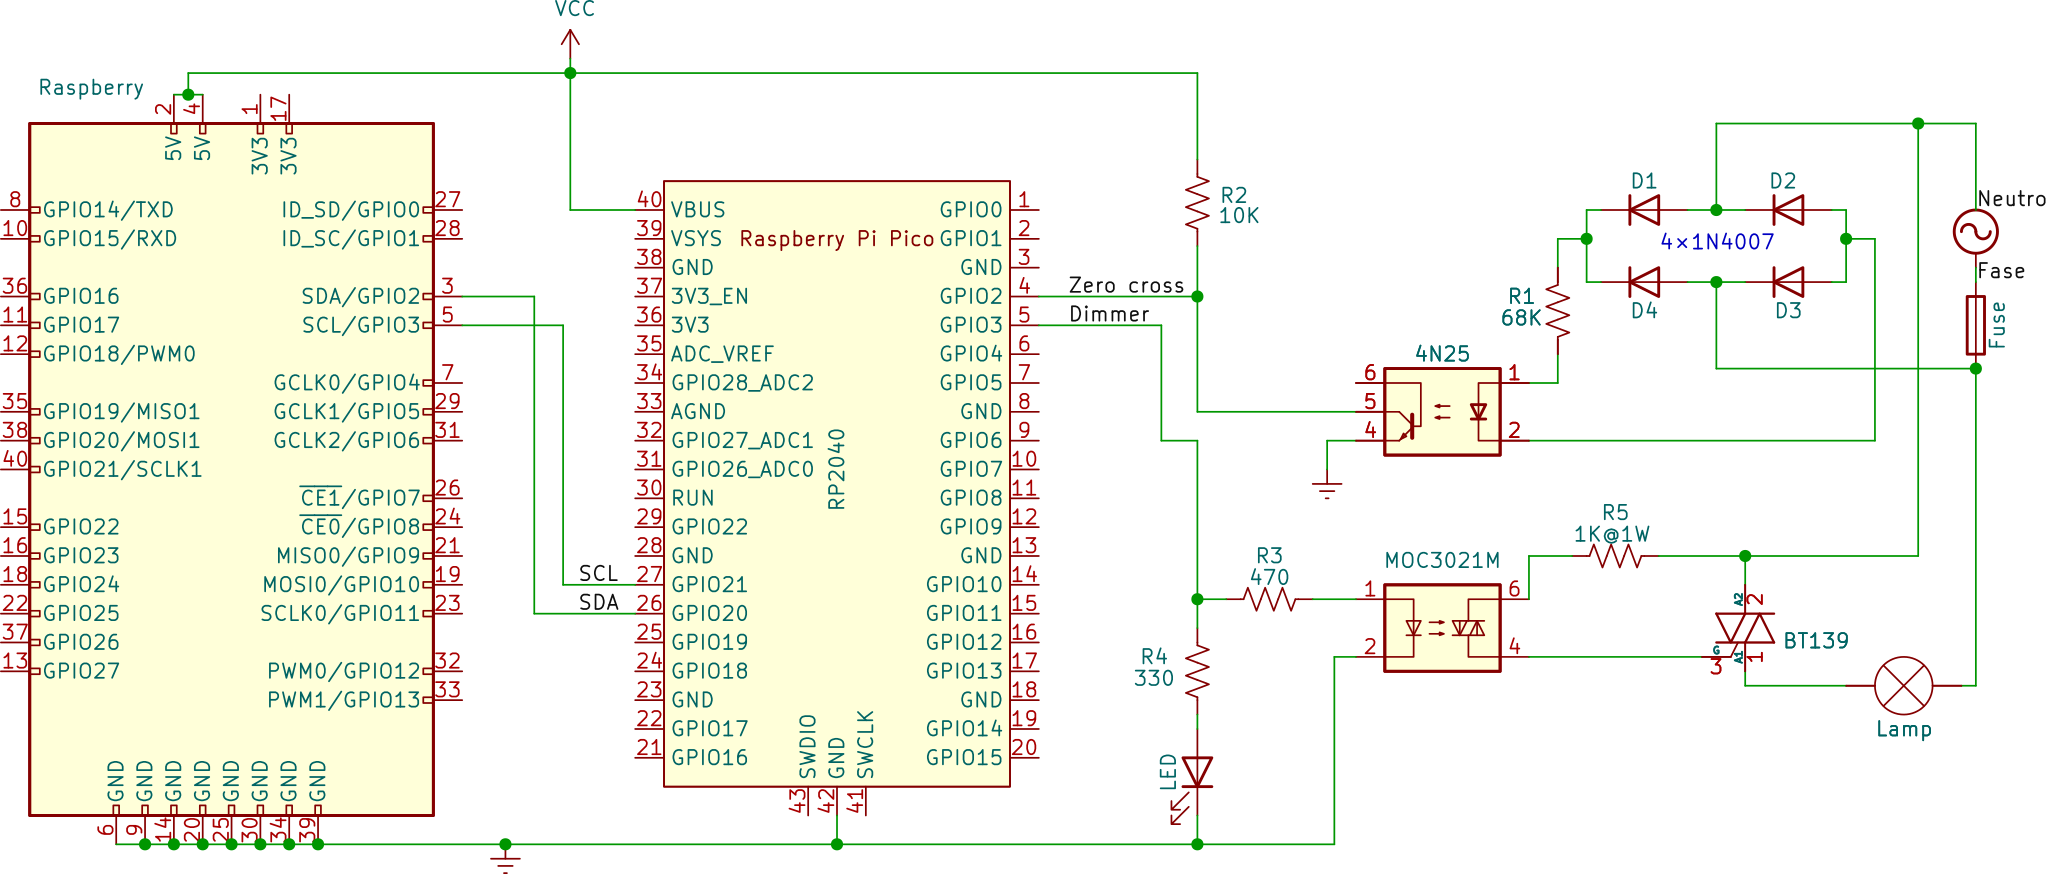
\includegraphics[width=0.85\linewidth,height=6cm,keepaspectratio]{img/circuit-full.png}
	\caption{Circuito AC-DC optoacoplado completo para control cerrado de temperatura.}%
	\label{fig:circuit-full}
\end{figure}

De acuerdo con el alambrado de la \Cref{fig:circuit-full}, el Arduino ha de realizar tres funciones:
\begin{enumerate*}[label=\roman*\rpar]
	\item digitalización del valor de temperatura analógico sensado por el LM35,
	\item la detección del cruce por cero de la onda sinusoidal de la línea eléctrica,
	y
	\item la modulación de potencia del foco incandescente mediante variación de fase ajustada por el retardo en el disparo del TRIAC.
\end{enumerate*}
Al igual que en las prácticas anteriores, el Arduino estará configurado como dispositivo esclavo y estas operaciones estarán al servicio del dispositivo maestro: la Raspberry Pi.
Así, una operación de lectura proporcionará al dispositivo maestro la temperatura sensada, mientras que una operación de escritura enviará la potencia con la que encenderá el foco como un valor flotante entre 0 y 100, quedando a cargo del Arduino el cálculo de la variación de fase y la sincronización de las operaciones de hardware.

\paragraph{Nota:} La implementación del código del Arduino se deja a cargo del estudiante.

\medskip

Se puede proceder entonces a revisar el código de control que se ejecutará en la Raspberry Pi.
En este caso se implementará un controlador On/Off tal como se describe en la \Cref{sec:control-onoff}.

Lo primero es incluir los paquetes necesarios y proveer cuatro parámetros importantes:
\begin{enumerate*}[label=\arabic*\rpar]
	\item la dirección del dispositivo esclavo,
	\item la temperatura deseada,
	\item el umbral o valor de encendido,
	y
	\item el umbral o valor de apagado
\end{enumerate*}
tal como se muestra en el \Cref{lst:controller-code-params}.

\begin{minipage}{\linewidth}%
\lstinputlisting[%
	language=python,
	caption={\texttt{controller-on-off.py:9--20} --- Parámetros},
	label={lst:controller-code-params},
	firstline=9,
	lastline=20]{src/controller-on-off.py}
\end{minipage}

El controlador con los parámetros descritos anteriormente requerirá de dos funciones auxiliares: \emph{readTemperature} (véase \Cref{lst:controller-code-read}) y \emph{writePower} (véase \Cref{lst:controller-code-write}).
La primer función corresponde a una operación de lectura en la cual el Arduino proporcionará la temperatura registrada por el sensor en grados centígrados codificado como un valor flotante (4 bytes en little endian).
La segunda función es una operación de escritura en la cual la Raspberry Pi proporcionará al arduino el factor de potencia de 0 a 100 codificada como un valor flotante (4 bytes en little endian).

\begin{minipage}{\linewidth}%
\lstinputlisting[%
	language=python,
	caption={\texttt{controller-on-off.py:26--36} --- Función \emph{readTemperature}},
	label={lst:controller-code-read},
	firstline=26,
	lastline=36]{src/controller-on-off.py}
\end{minipage}

\begin{minipage}{\linewidth}%
\lstinputlisting[%
	language=python,
	caption={\texttt{controller-on-off.py:38--45} --- Función \emph{writePower}},
	label={lst:controller-code-write},
	firstline=38,
	lastline=45]{src/controller-on-off.py}
\end{minipage}

Por último queda revisar la implementación del controlador mostrada en el \Cref{lst:controller-onoff-code}.
El control de temperatura se ejecuta en un bucle infinito de tres partes dentro de la función principal \emph{main}.
\begin{enumerate*}[label=\arabic*\rpar]
	\item Primero se lee la temperatura en °C del arduino,
	\item después esta se compara con los umbrales.
	Si la temperatura es menor al valor de encendido la lámpara se enciende a máxima potencia y permanecerá encendida hasta que se supera el valor de apagado.
	Por último,
	\item el controlador entra en un estado de espera (1 segundo) donde no se realiza ninguna acción.
\end{enumerate*}
En cualquier otro caso no se hace nada.

\begin{minipage}{\linewidth}%
\lstinputlisting[%
	language=python,
	caption={\texttt{controller-on-off.py:47--67} --- Función \emph{main}},
	label={lst:controller-onoff-code},
	linerange={47-47,51-52,54-55,57-67} %CHKTEX 8
	]{src/controller-on-off.py}
\end{minipage}
% %% %%%%%%%%%%%%%%%%%%%%%%%%%%%%%%%%%%%%%%%%%%%%%%%%%%%%%%%%%%
% step-2.tex
%
% Author:  Mauricio Matamoros
% License: MIT
%
% %% %%%%%%%%%%%%%%%%%%%%%%%%%%%%%%%%%%%%%%%%%%%%%%%%%%%%%%%%%%

%!TEX root = ../main.tex
%!TEX root = ../references.bib

\subsection{Paso 2: Led parpadeante}%
\label{sec:step2}
El código mostrado en \Cref{src:blink} muestra cómo se haría parpadear un LED mediante tiempos de espera o \emph{sleeps} utilizando la Raspberry Pi.

\smallskip
\lstinputlisting[%
	language=Python,
	linerange={18-40}, % chktex 8
	caption={\texttt{blink.py}},
	label={src:blink}
]{src/blink.py}
\smallskip

Estudie el código y véalo en funcionamiento, ejecutándolo de la siguiente manera:
\begin{Verbatim}[fontsize=\footnotesize]
./blink.py
\end{Verbatim}

% %% %%%%%%%%%%%%%%%%%%%%%%%%%%%%%%%%%%%%%%%%%%%%%%%%%%%%%%%%%%
% step-3.tex
%
% Author:  Mauricio Matamoros
% License: MIT
%
% %% %%%%%%%%%%%%%%%%%%%%%%%%%%%%%%%%%%%%%%%%%%%%%%%%%%%%%%%%%%
%!TEX root = ../practica.tex
%!TEX root = ../references.bib

% CHKTEX-FILE 1
% CHKTEX-FILE 13
% CHKTEX-FILE 46
\subsection{Paso 3: Control en lazo abierto de la potencia de una carga resistiva}%
\label{sec:step3}
Antes de proceder, verifique conexiones con un multímetro en busca de corto circuitos.
En particular verifique que los circuitos de AC y DC funcionan de manera independiente y que existe una impedancia infinita entre pines optoacoplados.

Con la Raspberry Pi configurada, basta con generar los dos programas para transferir la potencia de salida deseada de la Raspberry Pi al RP2040 que se encargará cortar el flujo de corriente en el instante correcto para obtener la potencia deseada.

Primero, es necesario configurar al RP2040 como dispositivo esclavo e inicializar el bus \IIC, tal como se muestra en el \Cref{lst:rp2040-test-i2c-setup}.
Las comunicaciones via \IIC son síncronas, lo que simplifica enormemente el diseño del programa.

\lstinputlisting[%
	language=Python,
	caption={\texttt{rp2040-test-i2c.py:23} --- Dirección asignada al dispositivo esclavo},
	label={lst:rp2040-test-i2c-setup},
	linerange=23-23]{src/rp2040-test-i2c.py} %CHKTEX 8

Tanto el envío como la recepción de datos se realizan byte por byte, por lo que es necesario convertir la potencia (\emph{float}) en un arreglo de bytes que pueda ser transmitido.
Para esta opreación se utilizará la librería \texttt{ustruct} que empaquetará y desempaquetará flotantes (\emph{float}) en listas de 4 bytes que pueden ser enviados o recibidos via \IIC de manera análoga a como se muestra en los \Cref{lst:rpi-code-i2c-read,lst:rpi-code-i2c-write}


Del lado de la Raspberry Pi, primero ha inicializarse el bus \IIC y posteriormente se realizarán las lecturas en un poleo o bucle infinito, cada una de las cuales se irá almacenando en un archivo bitácora.
La inicialización del bus requiere de una simple línea (véase \Cref{lst:rpi-code-i2c-setup}).

\lstinputlisting[%
	language=Python,
	caption={\texttt{raspberry-code-i2c.py:18} --- Configuración del bus \IIC},
	label={lst:rpi-code-i2c-setup},
	linerange=18-18]{src/raspberry-code-i2c.py} %CHKTEX 8

La conversión de un arreglo de bytes a punto flotante en Python no es inmediata.
Para esta opreación se utilizará la librería \texttt{struct} que empaquetará y desempaquetará flotantes (\emph{float}) en listas de 4 bytes que pueden ser enviados o recibidos del RP2040 via \IIC tal como se muestra en los \Cref{lst:rpi-code-i2c-read,lst:rpi-code-i2c-write}

\lstinputlisting[%
	language=Python,
	caption={\texttt{raspberry-code-i2c.py:36--43} --- Escritura de flotantes en el bus \IIC},
	label={lst:rpi-code-i2c-write},
	linerange=36-43]{src/raspberry-code-i2c.py} %CHKTEX 8

\lstinputlisting[%
	language=Python,
	caption={\texttt{raspberry-code-i2c.py:20--34} --- Lectura de flotantes del bus \IIC},
	label={lst:rpi-code-i2c-read},
	linerange=20-34]{src/raspberry-code-i2c.py} %CHKTEX 8


El resto del programa es trivial, pues consiste sólo en solicitar al usuario un valor de potencia y enviarlo al RP2040.

Por conveniencia, los códigos completos de los programas de ejemplo se encuentran en los \Cref{sec:appendix1,sec:appendix2,sec:appendix3,sec:appendix4}.

% %% %%%%%%%%%%%%%%%%%%%%%%%%%%%%%%%%%%%%%%%%%%%%%%%%%%%%%%%%%%
% step-4.tex
%
% Author:  Mauricio Matamoros
% License: MIT
%
% %% %%%%%%%%%%%%%%%%%%%%%%%%%%%%%%%%%%%%%%%%%%%%%%%%%%%%%%%%%%

%!TEX root = ../practica.tex
%!TEX root = ../references.bib

% CHKTEX-FILE 1
% CHKTEX-FILE 13
% CHKTEX-FILE 46

\subsection{Paso 4: Bitácora de temperatura via \IIC}%
\label{sec:step4}

Con la Raspberry Pi configurada, basta con generar los dos programas para transferir las temperaturas registradas en el Arduino a la Raspberry Pi que se encargará de almacenar esta información en un archivo o bitácora.

Primero, es necesario configurar al Arduino como dispositivo esclavo e inicializar el bus \IIC, tal como se muestra en los \Cref{lst:arduino-code-i2c-def,lst:arduino-code-i2c-setup}.
Las comunicaciones via \IIC son asíncronas, por lo que se requerirá almacenar la temperatura en una variable global que será leída por la función que atenderá las peticiones de datos del dispositivo maestro (la Raspberry Pi).

\lstinputlisting[%
	language=C,
	caption={\texttt{arduino-code-i2c.cpp:16} --- Dirección asignada al dispositivo esclavo},
	label={lst:arduino-code-i2c-def},
	firstline=16,
	lastline=16]{src/arduino-code-i2c.cpp}

\lstinputlisting[%
	language=C,
	caption={\texttt{arduino-code-i2c.cpp:37--42} --- Configuración del bus \IIC y funciones de control},
	label={lst:arduino-code-i2c-setup},
	firstline=37,
	lastline=42]{src/arduino-code-i2c.cpp}

El envío de datos se realiza byte por byte, por lo que es necesario convertir la medición de temperatura (\emph{float}) en un arreglo de bytes que pueda ser transmitido.
Esto se hace en la función \texttt{i2c\_request\_handler} con una llamada a \texttt{Wire.write} tal como se ilustra en el \Cref{lst:arduino-code-i2c-reqh}.

\lstinputlisting[%
	language=C,
	caption={\texttt{arduino-code-i2c.cpp:58--60} --- Envío asíncrono de datos},
	label={lst:arduino-code-i2c-reqh},
	firstline=56,
	lastline=58]{src/arduino-code-i2c.cpp}

Del lado de la Raspberry Pi, primero ha inicializarse el bus \IIC mediante el uso de la librería \texttt{smbus}\footnotemark y posteriormente se realizarán las lecturas en un poleo o bucle infinito, cada una de las cuales se irá almacenando en un archivo bitácora.
La inicialización del bus requiere de una simple línea (véase \Cref{lst:rpi-code-i2c-setup}).
\footnotetext{La implementación de la práctica utiliza \texttt{smbus2} que es una reimplementación codificada exclusivamente en Python de la librería \texttt{smbus} que es un \emph{wrapper} de la \emph{smbuslib} de C.}

\lstinputlisting[%
	language=Python,
	caption={\texttt{raspberry-code-i2c.py:26} --- Configuración del bus \IIC},
	label={lst:rpi-code-i2c-setup},
	linerange={9-10,19-21}% CHKTEX 8
	]{src/raspberry-code-i2c.py}

La conversión de un arreglo de bytes a punto flotante en Python no es inmediata.
Para esta opreación se utilizará la librería \texttt{struct} (véase \Cref{lst:rpi-code-i2c-setup}) que tomará los cuatro paquetes de 1 byte recibidos vía \IIC del Arduino y los convertira en un \emph{float}, como se muestra en el \Cref{lst:rpi-code-i2c-read}.
Nótese el símbolo $<$ (menor qué) a la izquierda del especificador de formato $f$, el cual se utiliza para definir el endianness de la transmisión de la información.

\lstinputlisting[%
	language=Python,
	caption={\texttt{raspberry-code-i2c.py:28--35} --- Lectura de flotantes del bus \IIC},
	label={lst:rpi-code-i2c-read},
	linerange={23-35} %CHKTEX 8
	]{src/raspberry-code-i2c.py}

El resto del programa es trivial, pues consiste sólo en la escritura del \emph{timestamp UNIX} y el valor de temperatura registrado en un archivo de texto y la lectura de datos del arduino cada segundo.

Por conveniencia, los códigos completos de los programas de ejemplo se encuentran en los \Cref{sec:appendix1,sec:appendix2,sec:appendix3}.

% %% %%%%%%%%%%%%%%%%%%%%%%%%%%%%%%%%%%%%%%%%%%%%%%%%%%%%%%%%%%
% step-4.tex
%
% Author:  Mauricio Matamoros
% License: MIT
%
% %% %%%%%%%%%%%%%%%%%%%%%%%%%%%%%%%%%%%%%%%%%%%%%%%%%%%%%%%%%%

%!TEX root = ../practica.tex
%!TEX root = ../references.bib

% CHKTEX-FILE 1
% CHKTEX-FILE 13
% CHKTEX-FILE 46

\subsection{Paso 5: Temperatura del RP2040}%
\label{sec:step5}

La \cref{eqn:v-to-temp} tiene un problema fundamental: un convertidor ADC entrega valores discretos enteros que corresponden de forma proporcional y lineal al voltaje sensado entre $V_\text{Ref-}$ y $V_\text{Ref+}$.
En el caso del RP2040 $V_\text{Ref-} = \text{\textsc{Gnd}} = 0\text{V}$ y $V_\text{Ref+} = \text{\textsc{Vcc}} = 3.3\text{V}$ y, dado que la precisión del ADC es de 12bits, los valores registrados estarrían entre cero y $2^{12}-1 = 4095$.
Sin embargo, MicroPython ofrece el método \code{read_u16()} de las instancias de \code{ADC} que provee un entero no signado de 16 bits.
Así, las conversiones tendrán que tomar en cuenta un rango entre 0 y 65535.

Con esto en mente y considerando que $v = \frac{3.3V}{65535}x$, se puede reemplazar $v$ por $x$ en la \cref{eqn:v-to-temp} para obtener una fórmula de conversión directa del valor reportado del ADC a un valor de temperatura.

\noindent
Así, la \cref{eqn:v-to-temp} quedaría como:

\begin{align*}%
	\label{eqn:adc-to-temp}
	T &=%
		\Bigg( \frac{-1}{1.721\frac{\text{mV}}{\text{°C}}} \Bigg)
		\Bigg( \frac{3.3\text{V}}{65535} \cdot x \Bigg) +
		437.23\text{°C} \\
%
	  &=
		\Bigg( \frac{-1}{1.721\frac{\text{mV}}{\text{°C}}} \Bigg)
		\Bigg( \frac{3300\text{mV}}{65535} \cdot x \Bigg) +
		437.23\text{°C} \\
%
	  &=
		\frac{
			-3300\cancel{\text{mV}}
		}{
			65535 \times 1.721\frac{\cancel{\text{mV}}}{\text{°C}}
		}
		\cdot x +
		437.23\text{°C} \\
%
	  &=
		\frac{
			-3300
		}{
			112785.74\frac{1}{\text{°C}}
		}
		\cdot x +
		437.23\text{°C} \\
\end{align*}

\noindent
Lo que finalmente produce la ecuación:

\begin{equation}%
	\label{eqn:adc-to-temp}
	T = -29259\times10^{-6}x + 437.23
\end{equation}

\noindent
Esta ley se refleja en el código presentado en \cref{lst:temp}.

\medskip{}

\noindent
Ingrese el siguiente código en el editor de Thonny y ejecútelo

\lstinputlisting[%
	language=Python,
	caption={\texttt{temp.py}: --- Temperatura del RP2040},
	label={lst:temp},
	firstline=11
]{src/temp.py}


El \cref{lst:temp} configura primero el ADC para leer del canal 4 (sensor interno de temperatura) y luego define un bucle infinito con la cláusula \code{while} dentro del cual
\begin{enumerate*}[label=\roman*\rpar]
	\item se lee el valor del convertidor A/D,
	\item se convierte el valor sensado a temperatura en grados celcius
	\item se imprime la temperatura
	y, finalmente,
	\item se espera durante un segundo.
\end{enumerate*}

Por conveniencia, los códigos completos de los programas de ejemplo se encuentran en el \Cref{sec:appendix3}.


\cleardoublepage
% %% %%%%%%%%%%%%%%%%%%%%%%%%%%%%%%%%%%%%%%%%%%%%%%%%%%%%%%%%%%
% experimens.tex
%
% Author:  Mauricio Matamoros
% License: MIT
%
% %% %%%%%%%%%%%%%%%%%%%%%%%%%%%%%%%%%%%%%%%%%%%%%%%%%%%%%%%%%%

%!TEX root = ../practica.tex
%!TEX root = ../references.bib

% CHKTEX-FILE 1
% CHKTEX-FILE 13
% CHKTEX-FILE 46

\section{Experimentos}%
\label{sec:experiments}

\begin{enumerate}
	\item{} [6pt] Modifique el código de la \cref{sec:step4} para que el brillo del led centinela se vea atenuado.
	\item{} [4pt] Modifique el código de la \cref{sec:step5} para que la temperatura se reporte tanto en grados Farenheit como en Centígrados.
% 	\item{} [4pt] Modifique el código de la \cref{sec:step4} la Raspberry Pi grafique el histórico de temperaturas registradas, leyendo los valores almacenados e ingresados en la bitácora.
	\item{} [+3pt] Con base en lo aprendido, modifique el código de la \cref{sec:step4} atenúe el brillo del led usando un PWM en lugar de retardos.
	\item{} [+2pt] Usando Thonny cargue un archivo \code{main.py} en el RP2040 para que su programa se inicie de forma automática y autónoma.
\end{enumerate}

\noindent
\textbf{Nota:} Anexe en su reporte las imágenes o enlaces a videos correspondientes a cada experimento como evidencia de su ejecución.

% %% %%%%%%%%%%%%%%%%%%%%%%%%%%%%%%%%%%%%%%%%%%%%%%%%%%%%%%%%%%
% references.tex
%
% Author:  Mauricio Matamoros
% License: MIT
%
% %% %%%%%%%%%%%%%%%%%%%%%%%%%%%%%%%%%%%%%%%%%%%%%%%%%%%%%%%%%%


%!TEX ROOT=../main.tex
%!TEX ROOT=../references.bib

% CHKTEX-FILE 1
% CHKTEX-FILE 46

\cleardoublepage
\section{Referencias}%
\label{sec:references}
\nocite{*}
\bibliographystyle{unsrtnat}
\bibliography{references}

\appendix

% %% %%%%%%%%%%%%%%%%%%%%%%%%%%%%%%%%%%%%%%%%%%%%%%%%%%%%%%%%%%
% appendices.tex
%
% Author:  Mauricio Matamoros
% License: MIT
%
% %% %%%%%%%%%%%%%%%%%%%%%%%%%%%%%%%%%%%%%%%%%%%%%%%%%%%%%%%%%%
%!TEX root = ../practica.tex
%!TEX root = ../references.bib

% CHKTEX-FILE 1
% CHKTEX-FILE 13
% CHKTEX-FILE 46

\cleardoublepage
\section{Programa Ejemplo: \texttt{rp2040-test-zx.py}}%
\label{sec:appendix1}
\lstinputlisting[language=Python,firstline=14]{src/rp2040-test-zx.py}

\cleardoublepage
\section{Programa Ejemplo: \texttt{rp2040-test-i2c.py}}%
\label{sec:appendix3}
\lstinputlisting[language=Python,firstline=15]{src/rp2040-test-i2c.py}

\cleardoublepage
\section{Programa Ejemplo: \texttt{raspberry-code-i2c.py}}%
\label{sec:appendix2}
\lstinputlisting[language=Python,firstline=9]{src/raspberry-code-i2c.py}

\cleardoublepage
\section{Programa Ejemplo: \texttt{rp2040-test-acdc.py}}%
\label{sec:appendix4}
\lstinputlisting[language=Python,firstline=14]{src/rp2040-test-zx.py}

\cleardoublepage
\section{Librería: \texttt{i2cslave.py}}%
\label{sec:appendix5}
\lstinputlisting[language=Python,firstline=24]{src/i2cslave.py}

\end{document}

